\section{Ejercicio 2 - El lote de Rolando}

Se escribió un lote de tareas para simular la siguiente situación:

\begin{itemize}
	\item Correr un algoritmo que hace un uso intensivo de la CPU por 100 ciclos sin realizar llamadas bloqueantes.
	\item Escuchar una canción, que realiza 20 llamadas bloqueantes con una duración variable entre 2 y 4 ciclos.
	\item Navegar por internet, que realiza 25 llamadas bloqueantes con una duración variable entre 2 y 4 ciclos.
\end{itemize}

Estas tareas se ponen a correr en el instante 0, 1 y 2 respectivamente, y Rolando espera que ejecuten en simultáneo.

\subsection{Pruebas}

Se ejecutó el simulador utilizando el algoritmo FCFS para 1 y 2 núcleos, con un cambio de contexto de 4 ciclos.  Las Figuras \ref{fig-rol1core} y \ref{fig-rol2core} muestran el resultado de ambas simulaciones.

\begin{figure}[!htb]
\begin{center}
  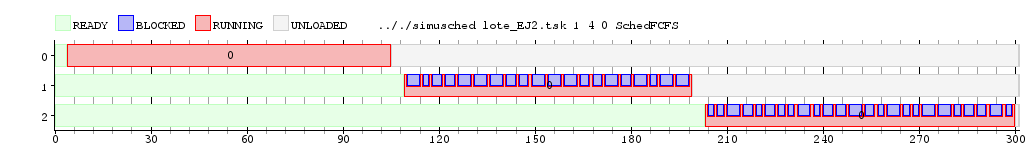
\includegraphics[scale=0.45]{imagenes/ej2-1core.png}
\end{center}
\caption{Simulación lote de Rolando con FCFS, 1 núcleo, 4 ciclos de cs}\label{fig-rol1core}
\end{figure}

\begin{figure}[!htb]
\begin{center}
  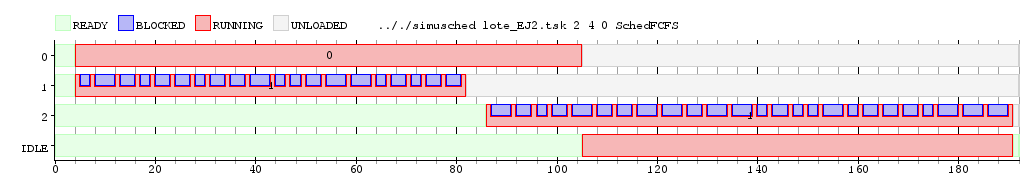
\includegraphics[scale=0.45]{imagenes/ej2-2core.png}
\end{center}
\caption{Simulación lote de Rolando con FCFS, 2 núcleos, 4 ciclos de cs}\label{fig-rol2core}
\end{figure}

En el caso de la Figura \ref{fig-rol1core}, la latencia de cada proceso es:

\begin{itemize}
	\item {\bf Tarea 0:} latencia 4
	\item {\bf Tarea 1:} latencia 108
	\item {\bf Tarea 2:} latencia 202
\end{itemize}

Estos valores nos dan un promedio aproximado de 30,3.
\vspace*{0.5cm}

Por otro lado, en el caso de la Figura \ref{fig-rol2core}, la latencia de cada proceso es:

\begin{itemize}
	\item {\bf Tarea 0:} latencia 4
	\item {\bf Tarea 1:} latencia 4
	\item {\bf Tarea 2:} latencia 83
\end{itemize}

Estos valores nos dan un promedio aproximado de 100,6.
\vspace*{0.5cm}

En el caso en el que Rolando se viera obligado a utilizar una computadora con un solo núcleo, como se utiliza un Sheduler del tipo FCFServe, no podría escuchar su canción preferida MIENTRAS corre el algoritmo, ya que las tres tareas se ejecutarán secuencialmente.  En el caso de poder utilizar una computadora con dos núcleos, podría correrse el algoritmo en uno de ellos y la canción en el otro, y Rolando podría trabajar a gusto.